\chapter{Funzionalità sviluppate}
\label{cap:funzionalità-sviluppate}

\section{Evidenziazione delle parole chiave}
\label{sec:highlight-keyword}

\par La funzionalità “Highlight Keywords” consente di evidenziare tutte le occorrenze di una parola chiave all’interno della pagina web in cui l’estensione è attiva. Ogni occorrenza viene formattata con colori di sfondo, testo e bordo differenti, in base al tag \gls{html} che la contiene; tali colori sono personalizzabili tramite le impostazioni dell’estensione. Oltre alla personalizzazione cromatica delle occorrenze, ciascuna di esse è accompagnata da un’etichetta, posizionata in alto a sinistra, che riporta il nome del tag genitore. Nell’interfaccia grafica, a ogni parola chiave è associato un pulsante (highlighter) che permette di attivare o disattivare l’evidenziazione a livello globale. Questa funzionalità è accessibile sia dalla pagina principale sia da quella dedicata a una singola keyword, e lo stato del pulsante rimane sincronizzato tra le due. Le parole chiave inserite manualmente dall'utente possono essere evidenziate anche prima dell’avvio dell’analisi vera e propria, tramite il pulsante dedicato, mantenendo le funzionalità di analisi ed evidenziazione separate e indipendenti.

\subsection{Problematiche riscontrate}

\par La prima difficoltà è stata individuare un metodo efficiente per navigare il \gls{dom}, escludendo al contempo gli elementi non rilevanti dal punto di vista \gls{seo}. Tra le opzioni considerate, l’oggetto \textit{TreeWalker} si è dimostrato il più adatto, in quanto permette di gestire in modo centralizzato la logica di filtraggio dei nodi, determinando in modo preciso quali accettare o scartare. La sfida successiva ha riguardato la definizione del criterio di ricerca delle parole chiave. A differenza di strumenti come \textit{MozBar}, ho scelto di non evidenziare le occorrenze che compaiono come sottostringhe all’interno di parole più lunghe (ad esempio “Java” all’interno di “JavaScript”). In fase di ricerca, parole separate da un punto, un trattino (alto o basso) o un apostrofo vengono considerate un’unica parola. Tutti gli altri caratteri sono trattati come separatori, in modo analogo a quanto avviene nell’estensione \textit{SEOquake}.

\vspace{10pt}
\par\noindent Una volta individuate le occorrenze di una parola chiave, l’evidenziazione è stata applicata utilizzando un oggetto \textit{DocumentFragment}, che permette di costruire in modo sicuro una struttura temporanea da inserire nel DOM principale. Per rimuovere l’evidenziazione e ripristinare correttamente il contenuto originale, è stata eseguita un’operazione di normalizzazione del DOM, tramite la quale i nodi di testo adiacenti vengono unificati e quelli vuoti rimossi.

\vspace{10pt}
\par\noindent Un altro ostacolo, particolarmente critico per l’affidabilità e le prestazioni del sistema, è emerso nel trattamento delle parole chiave composte da più termini separati da spazi (note anche come keyphrase). L’approccio iniziale prevedeva l’esecuzione della ricerca sui singoli nodi di testo; di conseguenza, una keyword come “JavaScript Tutorial” non veniva riconosciuta se i due termini erano distribuiti su tag distinti (ad esempio, un h1 e uno span annidato). Questo limite è stato rilevato nel corso di test manuali condotti su un blog di intrattenimento e informazione, che adotta una convenzione particolare: evidenziare in grassetto solo il cognome all’interno dei nomi propri. Ciò comportava la frammentazione di molte keyphrase, che non venivano identificate correttamente dal sistema. Per rendere la ricerca delle keyphrase più granulare e accurata, ho sviluppato due algoritmi: uno ricorsivo e uno iterativo. Il primo suddivide la keyphrase in blocchi e cerca ciascun blocco all’interno di nodi di testo adiacenti. Il secondo, invece, costruisce un testo virtuale concatenando il contenuto di nodi adiacenti, simulando il comportamento delle proprietà \textit{innerText} o \textit{textContent}. In entrambi gli approcci, i nodi adiacenti devono appartenere allo stesso contesto, ovvero condividere lo stesso elemento genitore ed essere elementi \textit{inline} validi (ad esempio strong, em, ecc.). Tra le due soluzioni, ho preferito il secondo algoritmo, in quanto più flessibile e maggiormente coerente con il comportamento reale del browser.

\vspace{10pt}
\par\noindent Nel secondo algoritmo, ogni volta che si concatena il contenuto di un nodo al testo virtuale, è necessario effettuare una mappatura degli indici di inizio e fine, in modo da poter risalire al nodo originale nel momento in cui vengono trovati \textit{match}. Questa operazione può risultare complessa, soprattutto in presenza di \gls{dom} profondi o fortemente nidificati. Per questo motivo, l’algoritmo “a nodi multipli” non ha sostituito quello originale, che esegue la ricerca sui singoli nodi di testo, ma coesiste con esso all’interno del sistema. I due algoritmi vengono richiamati dinamicamente in base alla tipologia di parola chiave: per le keyword semplici viene utilizzato l’algoritmo “a nodo singolo”, mentre per le keyphrase viene impiegato l’algoritmo “a nodi multipli”. È stato valutato anche il caso limite in cui una keyword semplice risulti spezzata su più tag. Tuttavia, trattandosi di una situazione molto rara, si è deciso di non complicare ulteriormente il flusso di ricerca per gestirla.

\begin{figure}[H]
  \centering 
  \fbox{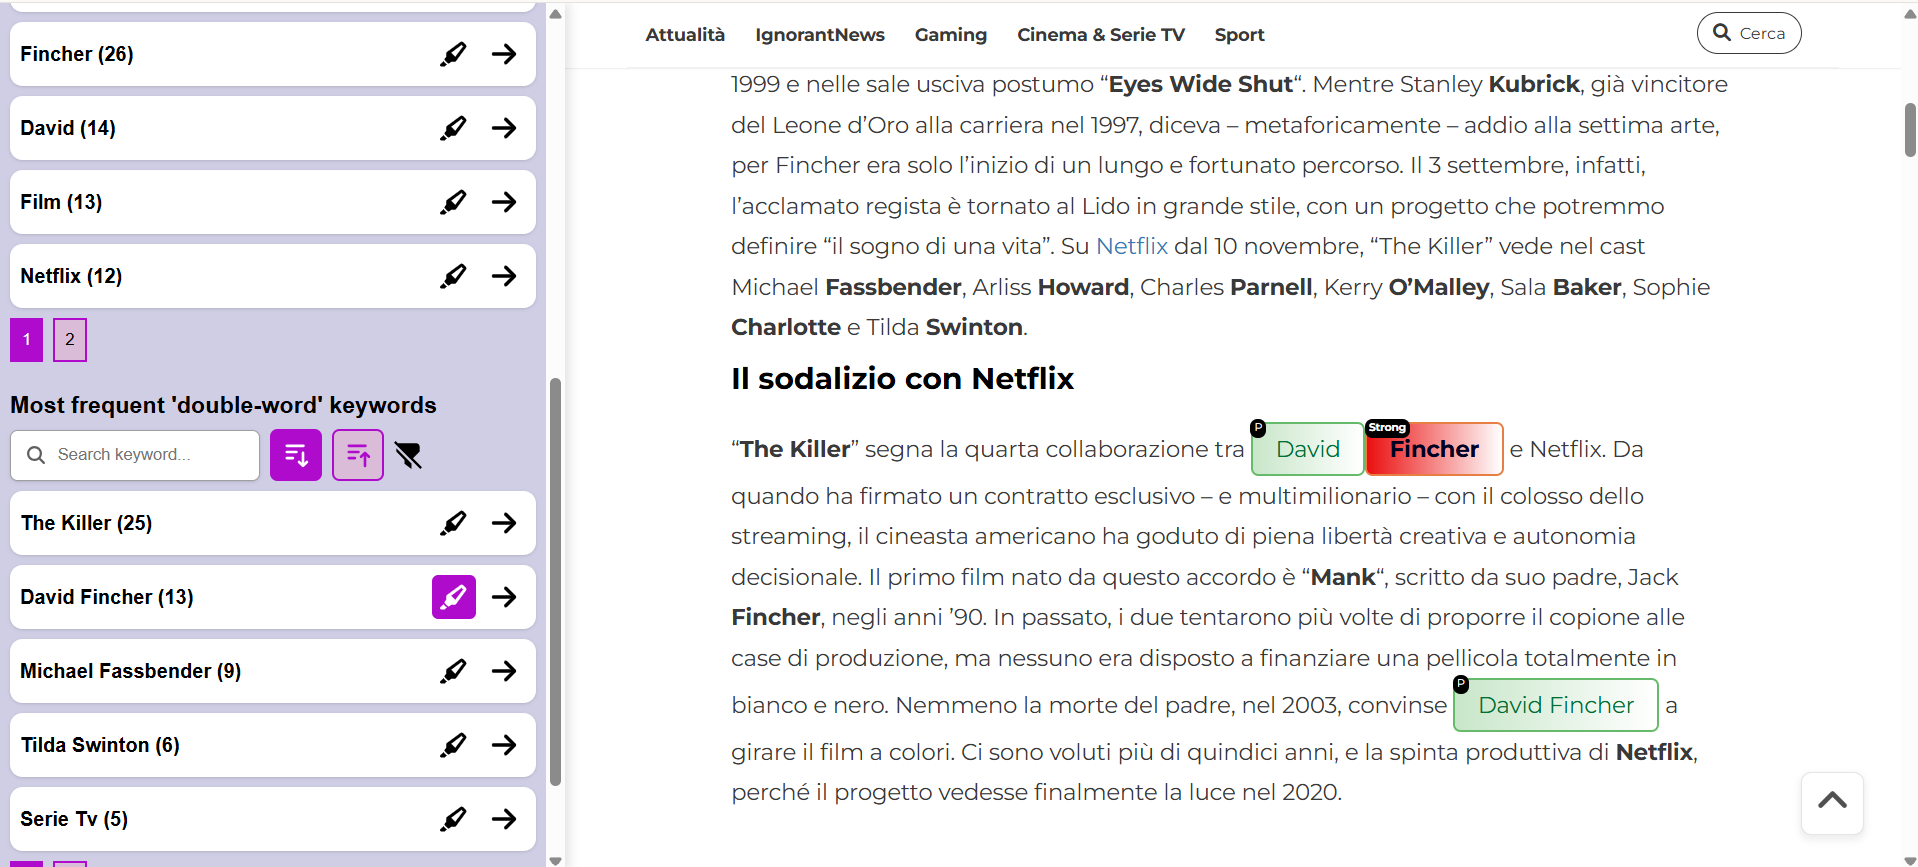
\includegraphics[width=0.95\columnwidth]{funzionalita/highlight.png}} 
  \caption{Evidenziazione delle parole chiave}
\end{figure}

\section{Analisi delle parole chiave}
\label{sec:analyze-keyword}

\par La funzionalità “Analyze Keywords” è stata progettata per operare principalmente su pagine web in lingua inglese e italiana. Questa funzionalità fornisce una panoramica generale dell'analisi \gls{on-page}, che include i seguenti elementi:
\begin{itemize}
  \item Contenuto del meta tag keywords;
  \item Lingua dichiarata nella pagina;
  \item Conteggio totale delle parole;
  \item Conteggio delle parole uniche.
\end{itemize}

\vspace{5pt}
\par\noindent Queste informazioni costituiscono la base per l'analisi delle parole chiave, che prende in considerazione diversi parametri, come la frequenza, la densità e il numero di occorrenze all’interno di un insieme predefinito di tag \gls{html}. L'analisi viene eseguita su una copia statica del \gls{dom}, al fine di garantire coerenza tra tutte le parole chiave, e può essere aggiornata manualmente tramite un pulsante dedicato. La ricerca delle parole chiave segue gli stessi criteri illustrati nella \hyperref[sec:highlight-keyword]{sezione \textsection\ref*{sec:highlight-keyword}}.

\vspace{10pt}
\par\noindent I tag semantici considerati più rilevanti dal punto di vista \gls{seo} sono:
\begin{itemize}
  \item Il tag title;
  \item Il meta tag description;
  \item I tag di intestazione (H1-H6);
  \item I paragrafi (<p>);
  \item I link (<a>);
  \item Il testo in grassetto (<strong>);
  \item Il test in corsivo (<em>);
  \item Le voci degli elenchi (<li>);
  \item Il testo alternativo delle immagini (Alt).
\end{itemize}

\vspace{5pt}
\par\noindent Per il calcolo delle occorrenze di una parola chiave all’interno di questi tag, sono stati adottati due approcci:
\begin{itemize}
  \item Accedere direttamente ai tag e utilizzare la proprietà textContent per estrarne il contenuto da analizzare;
  \item Risalire ai tag durante la navigazione del DOM con \textit{TreeWalker}, registrando le occorrenze contestualmente al calcolo della frequenza complessiva.
\end{itemize}

\vspace{5pt}
\par\noindent Poiché entrambi gli approcci sono stati considerati ugualmente validi, ho adottato il design pattern comportamentale \textit{Strategy}, in modo da poter selezionare dinamicamente l’algoritmo senza alterare il codice del modulo di analisi.

\subsection{Problematiche riscontrate}

\par Una delle difficoltà incontrate ha riguardato il calcolo di un punteggio da associare a ciascuna parola chiave. Le due opzioni considerate erano l’assegnazione di un punteggio di qualità o, in alternativa, di un punteggio basato sulla rilevanza strutturale. Tuttavia, in entrambi i casi è emerso che i criteri effettivamente utilizzati dai motori di ricerca sono molto più articolati e difficili da replicare in modo attendibile. Per questo motivo, ho concordato con la Proponente di non introdurre alcun sistema di punteggio.

\vspace{10pt}
\par\noindent Un’altra problematica è stata riscontrata in seguito alla modifica della modalità di analisi, con il passaggio dal \gls{dom} live a una copia statica. Durante l’operazione di clonazione, infatti, gli stili applicati agli elementi non vengono mantenuti, rendendo meno preciso il controllo sui tag \textit{inline} rispetto a quanto avviene nella funzionalità di evidenziazione, che opera direttamente sul DOM live. Tuttavia, in fase di analisi, è possibile fare affidamento sulla natura semantica dei tag \gls{html}. Pertanto, un controllo basato sul nome del tag risulta sufficiente nella maggior parte dei casi, garantendo un buon livello di affidabilità anche senza una verifica esplicita dello stile.

\vspace{10pt}
\par\noindent Un aspetto che ha generato ambiguità è stata la discrepanza tra la frequenza complessiva e la somma delle occorrenze rilevate nei singoli tag. Tale divergenza era dovuta al fatto che alcune occorrenze di una parola chiave si trovavano all’interno di tag annidati. La soluzione concordata con la Proponente è stata l’inserimento di un messaggio esplicativo, al fine di chiarire il comportamento del sistema ed evitare fraintendimenti da parte dell’utente.

\begin{figure}[H]
  \centering 
  \fbox{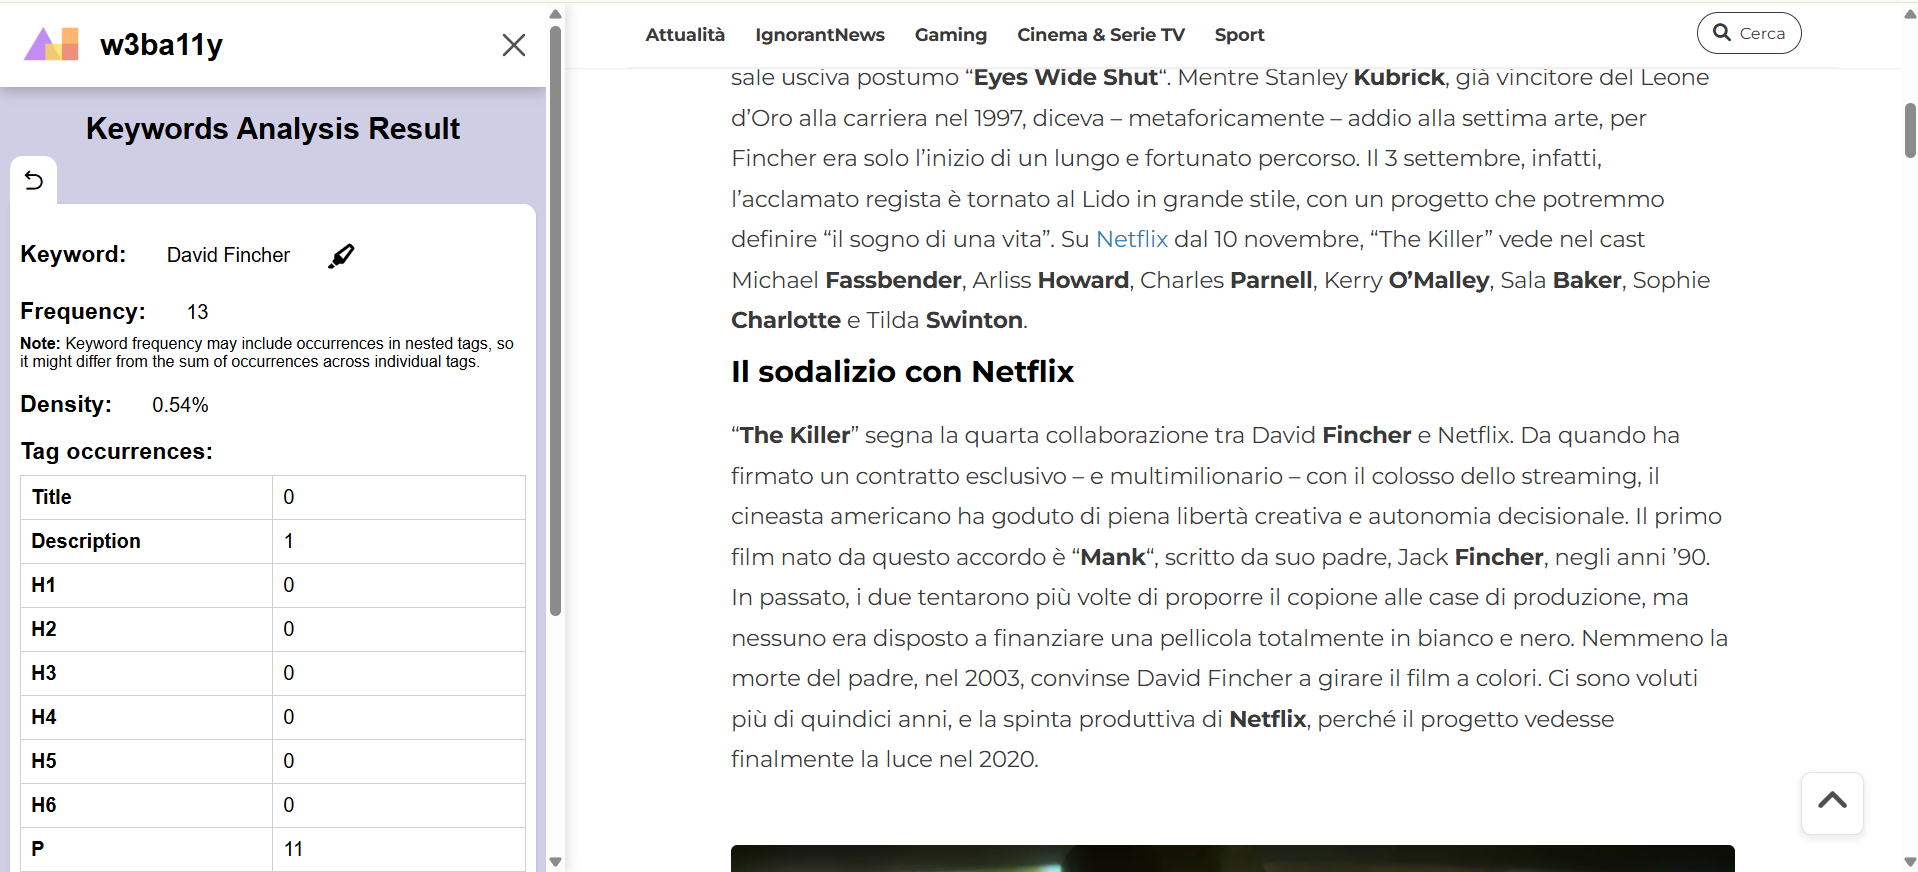
\includegraphics[width=0.95\columnwidth]{funzionalita/analysis.png}} 
  \caption{Analisi delle parole chiave}
\end{figure}

\section{Conteggio delle parole ed estrazione di quelle più frequenti}
\label{sec:count-word}

\par Il conteggio delle parole presenti nella pagina rappresenta un requisito fondamentale per il calcolo della densità di una keyword. L'estrazione delle parole dal testo avviene secondo un pattern che segue gli stessi criteri descritti nella \hyperref[sec:highlight-keyword]{sezione \textsection\ref*{sec:highlight-keyword}}. Tra i requisiti opzionali figura invece l'identificazione delle parole più frequenti, suddivisibili in categorie come “single-word”, “double-word” e così via. Questa funzionalità risulta particolarmente utile qualora il meta tag keywords non sia presente, poiché consente di suggerire all’utente un elenco di termini che, in base alla frequenza, possono essere considerati potenziali parole chiave. Il sistema seleziona le 10 parole più ricorrenti per ciascuna categoria, presentandole in ordine decrescente.

\subsection{Problematiche riscontrate}

\par Le \gls{stopword} devono essere escluse dal processo di identificazione delle parole più frequenti, in quanto non hanno valore semantico e difficilmente corrispondono a parole chiave. A tal fine, ho utilizzato una libreria esterna per definire una serie di liste di stopword, selezionate dinamicamente in base alla lingua dichiarata nella pagina. Nel caso delle “single-word”, l’esclusione delle stopword è diretta e immediata. La gestione delle espressioni composte da due o più termini (n-grammi), invece, richiede maggiore attenzione. Nei testi in lingua italiana, ad esempio, è piuttosto comune l’uso di termini o espressioni in inglese (lingua di riferimento a livello internazionale). In questi contesti, espressioni come “The Batman” possono essere considerate valide, mentre sequenze prive di valore semantico come “of the” andrebbero escluse. Per trattare in modo adeguato queste situazioni, ho implementato un duplice controllo: escludere tutte le stopword relative alla lingua dichiarata nella pagina e tollerare la presenza di stopword inglesi solo se queste non superano il 50\% dei termini dell’espressione.

\begin{figure}[H]
  \centering 
  \fbox{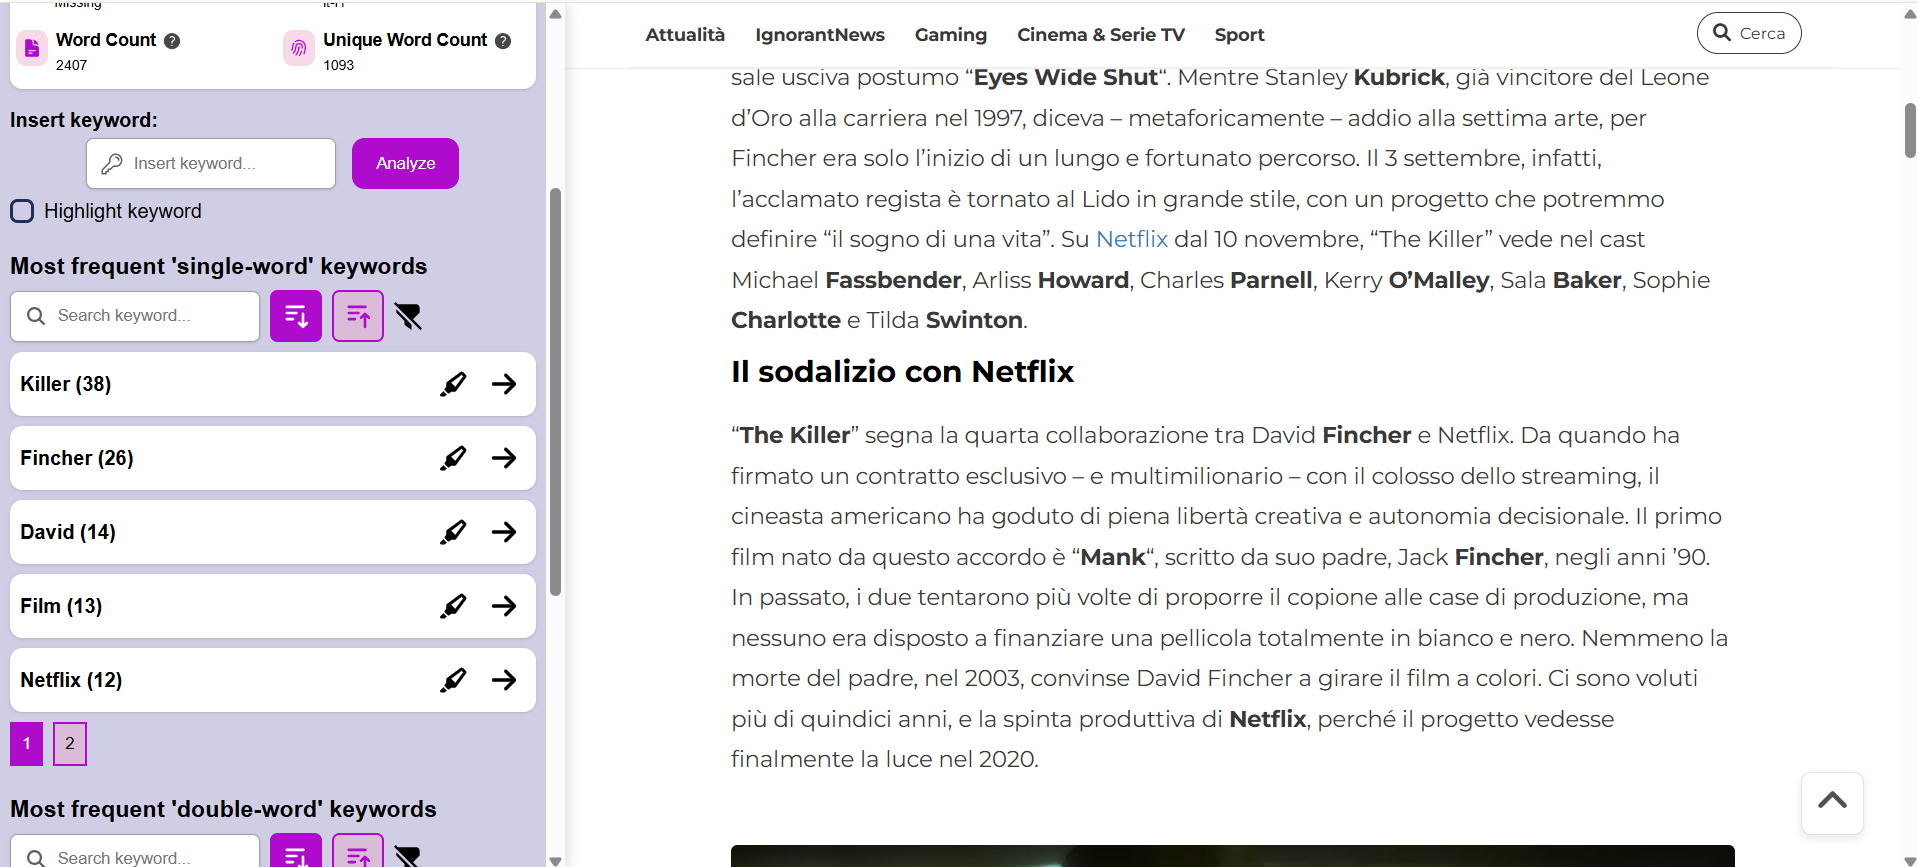
\includegraphics[width=0.95\columnwidth]{funzionalita/word_count.png}} 
  \caption{Conteggio delle parole chiave ed estrazione di quelle più frequenti}
\end{figure}

\section{Elenco delle parole chiave}
\label{sec:keyword-list}

\par L'interfaccia grafica è organizzata in quattro elenchi distinti: 
\begin{itemize}
  \item \textbf{Meta keywords}: parole chiave estratte dal meta tag keywords;
  \item \textbf{User-added keywords}: parole chiave inserite manualmente dall'utente;
  \item \textbf{Most frequent “single-word” keywords}: le 10 parole chiave più frequenti composte da un solo termine;
  \item \textbf{Most frequent “double-word” keywords}: le 10 parole chiave più frequenti composte da due termini.
\end{itemize}

\vspace{5pt}
\par\noindent Ogni elenco può essere ordinato per frequenza, filtrato per nome e ripristinato tramite appositi pulsanti. All’interno di ciascuna lista, il sistema carica 5 elementi alla volta, navigabili attraverso un sistema di paginazione. Per evitare di sovraccaricare l’interfaccia, non vengono mostrati tutti i pulsanti di navigazione delle pagine, ma solo un sottoinsieme calcolato dinamicamente secondo le seguenti regole:
\begin{itemize}
  \item Il pulsante per accedere alla prima pagina è sempre visibile;
  \item Il pulsante per accedere all’ultima pagina è sempre visibile;
  \item Sono visibili i due pulsanti precedenti a quello attualmente attivo;
  \item Sono visibili i due pulsanti successivi a quello attualmente attivo;
  \item I pulsanti nascosti sono sostituiti dalla stringa “...”.
\end{itemize}

\vspace{5pt}
\par\noindent A ciascuna parola chiave è associata un’indicazione della frequenza e un gruppo di pulsanti che consentono di eseguire operazioni come l’eliminazione, l’evidenziazione visiva e la visualizzazione dei risultati dell’analisi.

\subsection{Problematiche riscontrate}

\par L’elenco delle parole chiave più frequenti viene visualizzato, per impostazione predefinita, in ordine decrescente. Di conseguenza, il relativo pulsante di ordinamento deve risultare attivo sin dall’inizio. Una volta rimossi eventuali filtri, è necessario ripristinare il comportamento predefinito, ovvero riattivare il pulsante di ordinamento in modalità “desc”. Questa condizione è rimasta inosservata fino all’esecuzione dei test manuali, rendendo necessario un leggero \textit{refactoring} per evitare potenziali situazioni di disorientamento per l’utente.

\begin{figure}[H]
  \centering 
  \fbox{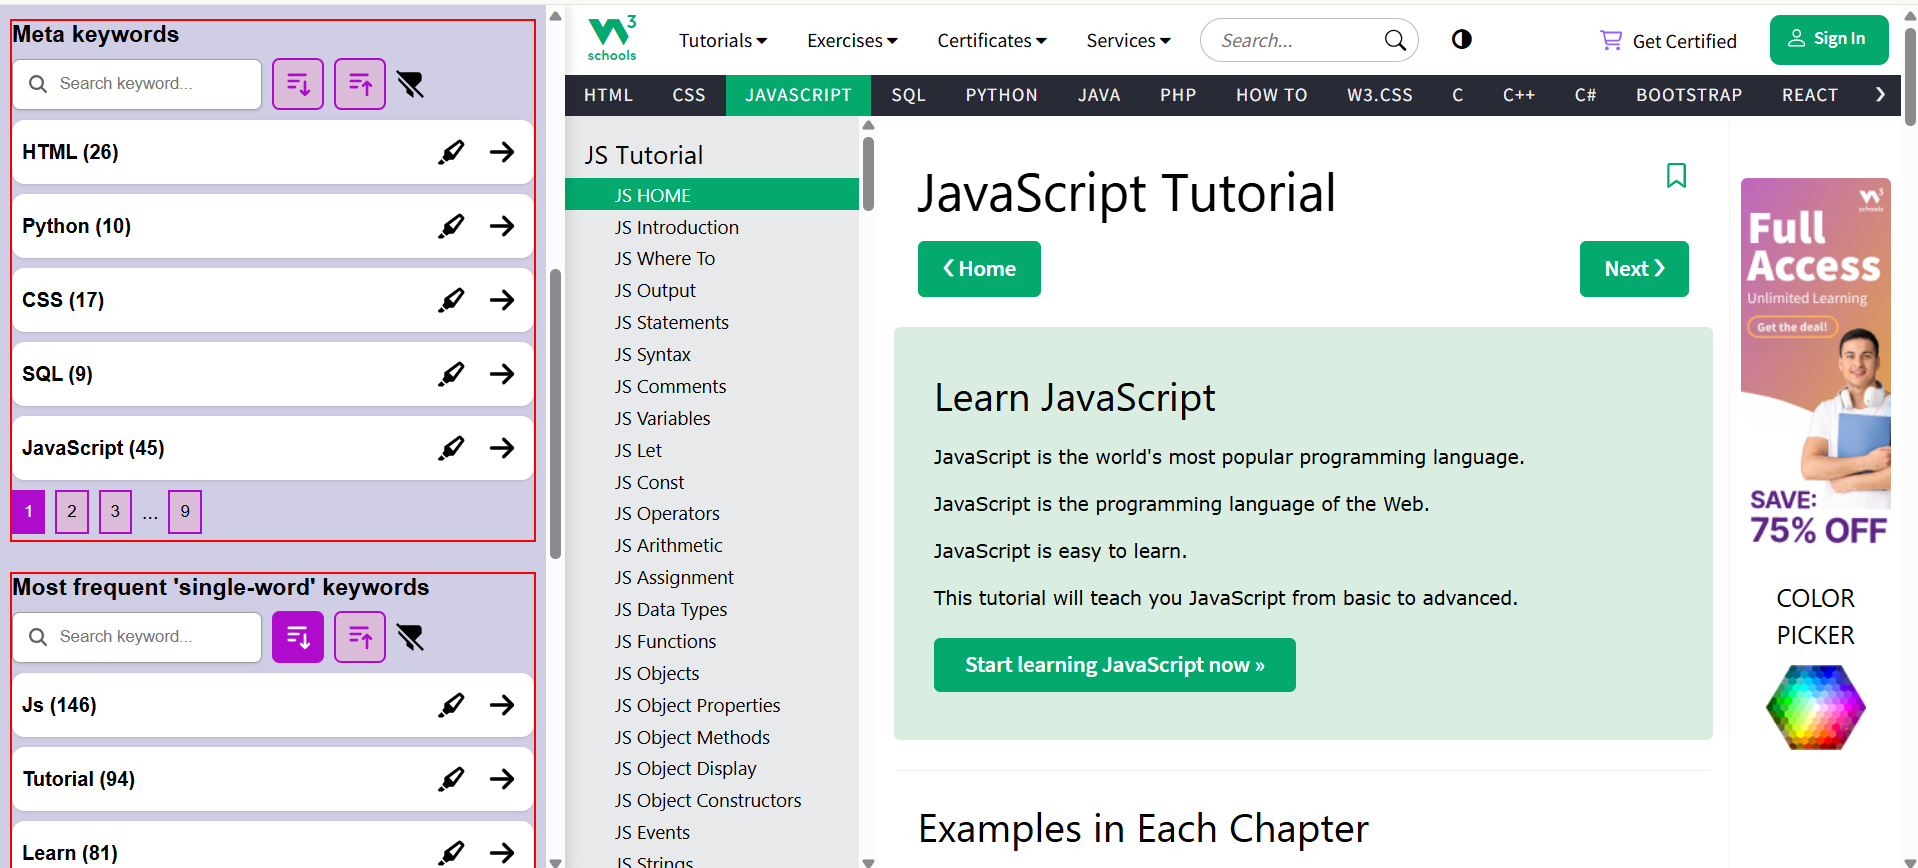
\includegraphics[width=0.95\columnwidth]{funzionalita/keyword_list.png}} 
  \caption{Elenco delle parole chiave}
\end{figure}

\section{Accessibilità}

\par Dal momento che la funzionalità di analisi delle parole chiave è integrata in un’estensione preesistente orientata all’accessibilità, anche questa componente è stata progettata in conformità alle linee guida \gls{wcag}. A tal fine, sono stati condotti test di accessibilità con i seguenti obiettivi:
\begin{itemize}
  \item Verificare il rispetto del \textbf{rapporto minimo di contrasto} tra testo e sfondo, pari a 4.5:1 per il testo di dimensioni “normali” e 3:1 per il testo di grandi dimensioni. Questo controllo è stato applicato sia agli elementi interni all’estensione, sia a quelli utilizzati per evidenziare le parole chiave;
  \item Controllare che le \textbf{immagini non decorative} siano dotate di un testo alternativo;
  \item Accertarsi che le \textbf{icone non decorative} siano accompagnate da un’etichetta accessibile;
  \item Verificare l’accessibilità dei \textbf{tooltip}, assicurandosi che vengano attivati e disattivati correttamente quando si interagisce con l’elemento trigger, sia tramite navigazione da tastiera sia tramite l’uso del mouse. Inoltre, i tooltip devono rimanere visibili al passaggio del mouse su di essi e devono poter essere chiusi premendo il tasto Esc;
  \item Controllare che tutti gli \textbf{elementi interattivi} (come pulsanti o link) dispongano di un’etichetta testuale descrittiva;
  \item Assicurare la \textbf{navigazione tramite tastiera}, con un ordine di tabulazione logico e una chiara indicazione visiva dell’elemento attualmente attivo.
\end{itemize}
